\begin{frame}{Định nghĩa}
    \begin{figure}[H] % places figure environment here   
        \centering % Centers Graphic
        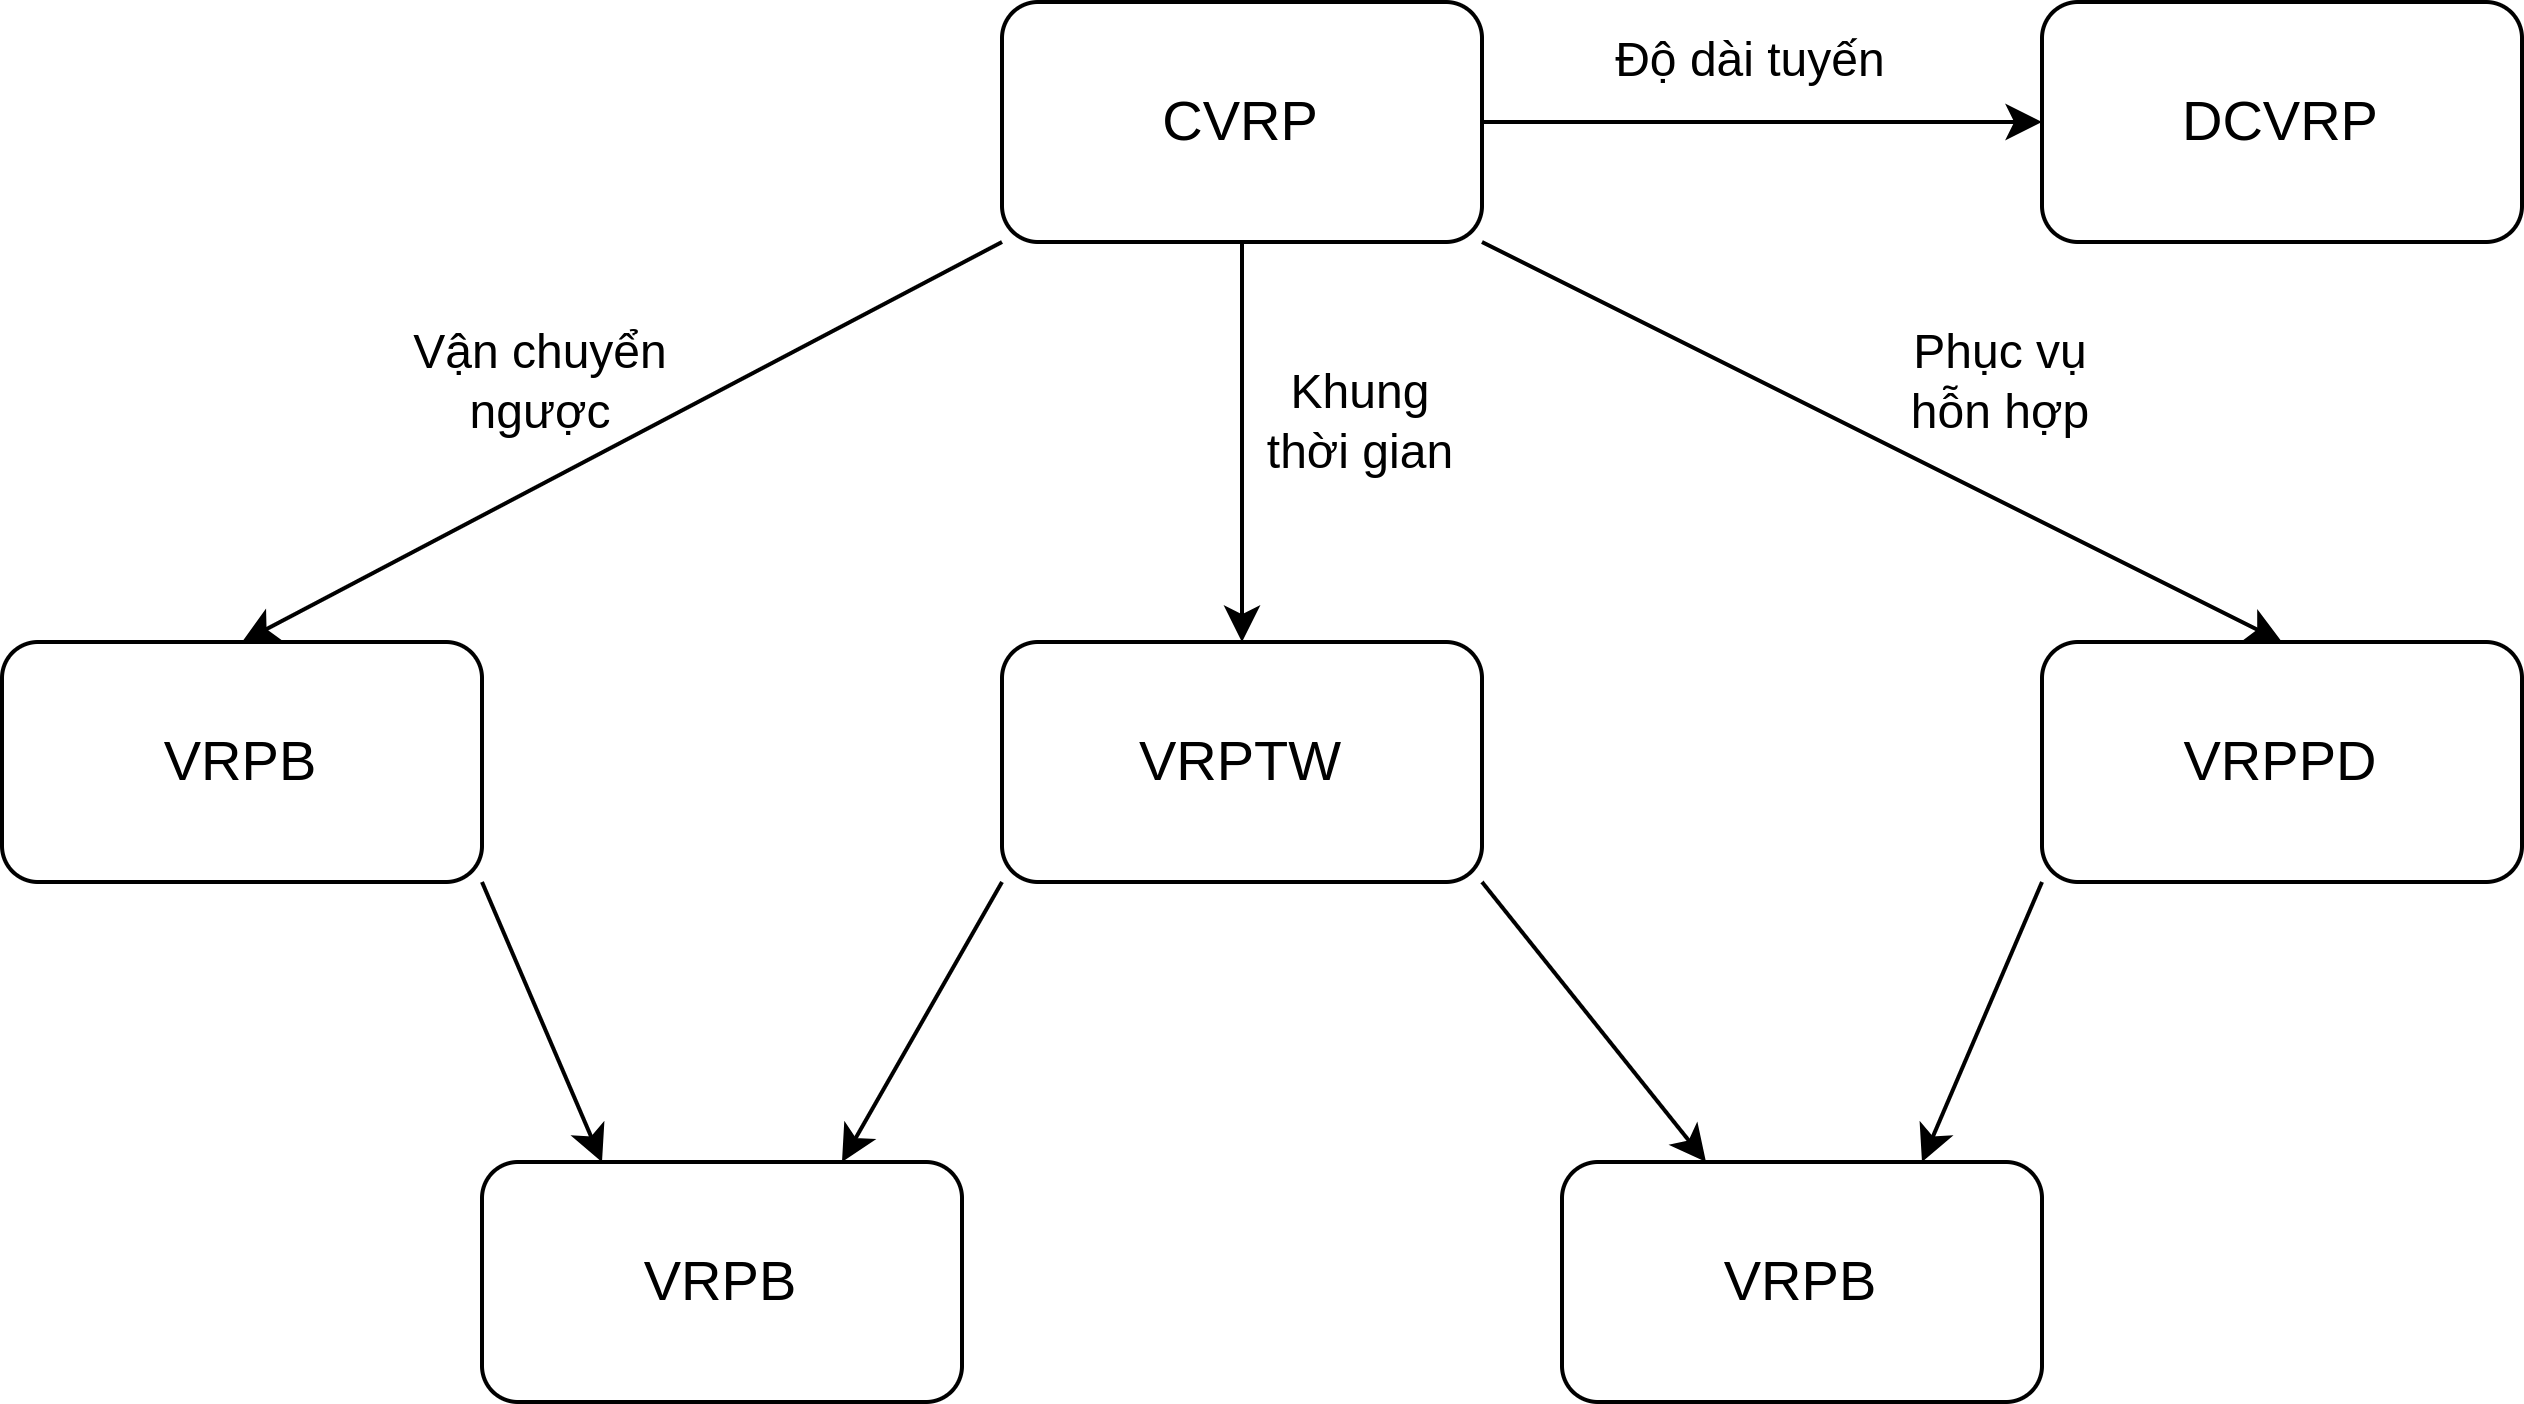
\includegraphics[width=0.8\textwidth]{figures/vrp.png} 
        \caption{Các bài toán, biến thể của VRP} % Creates caption underneath graph
        \label{fig:fg_01}
      \end{figure}
\end{frame}


\begin{frame}{Mô hình - Dòng xe}
    \textbf{Công thức dòng xe hai chỉ số }\\
    $x_{ij}$ nhận giá trị bằng $1$ nếu cung $(i, j) \in A$ nằm trong nghiệm tối ưu và $0$ nếu trong trường hợp còn lại.
    \begin{equation} \label{eq:vrp1}
        \text{(VRP1)} \quad \min \sum_{i \in V} \sum_{j \in V} c_{ij} x_{ij}
      \end{equation}
      s.t.
      \begin{flalign}
          \label{ct_vrp1:1}  & \sum_{i \in V} x_{ij} = 1 \quad \forall j \in V \setminus \{0\}, \\
        \label{ct_vrp1:2}  & \sum_{j \in V} x_{ij} = 1 \quad \forall i \in V \setminus \{0\}, \\
        \label{ct_vrp1:3}  & \sum_{i \in V} x_{i0} = K,
    \end{flalign}
\end{frame}

\begin{frame}{Mô hình - Dòng xe}
    \begin{flalign}
        \label{ct_vrp1:4}  & \sum_{j \in V} x_{0j} = K, \\
        \label{ct_vrp1:5}  & \sum_{i \notin  S} \sum_{j \in S} x_{ij} \geq r(S) \quad \forall S \subseteq V \setminus \{0\}, S \neq \emptyset, \\
        \label{ct_vrp1:6}  & x_{ij} \in \{0,1\} \quad \forall i,j \in V.
    \end{flalign}
\end{frame}

\begin{frame}{Mô hình - VRPTW}
    \textbf{Công thức dòng xe ba chỉ số }\\
    $x_{ijk}$ nhận giá trị 1 nếu xe $k$ đi trực tiếp từ nút $i$ tới nút $j$ và 0 nếu ngược lại.
    \begin{equation} \label{eq1}
        \min \sum_{k \in K} \sum_{(i,j) \in A} c_{ij} x_{ijk}
    \end{equation}
    s.t.
    \begin{flalign}
        \label{ct:1}  & \sum_{k \in K} \sum_{j \in \Delta^+(i)} x_{ijk} = 1 \quad \forall i \in N, \\
        \label{ct:2}  & \sum_{j \in \Delta^+(0)} x_{0jk} = 1 \quad \forall k \in K,                   \\
        \label{ct:3}  & \sum_{i \in \Delta^-(j)} x_{ijk} -  \sum_{i \in \Delta^+(j)} x_{jik} = 0 \quad \forall k \in K, j \in N,
    \end{flalign}
\end{frame}

\begin{frame}
    \begin{flalign}
        \label{ct:4}  & \sum_{i \in \Delta^-(n+1)} x_{i,n+1,k} = 1 \quad \forall k \in K, \\
        \label{ct:5}  & x_{ijk} (w_{ik} + s_i + t_{ij} - w_{jk}) \leq 0 \quad \forall k \in K, (i,j) \in A, \\
        \label{ct:6}  & a_i \sum_{j \in \Delta^+(i)} x_{ijk} \leq w_{ik} \leq b_i \sum_{j \in \Delta^+(i)} x_{ijk} \quad \forall k \in K, i \in N, \\
        \label{ct:7}  & E \leq w_{ik} \leq L \quad \forall k \in K, i \in \{0, n+1\}, \\
        \label{ct:8}  & \sum_{i \in N} d_i \sum_{j \in \Delta^+(i)} x_{ijk} \leq C \quad \forall k \in K, \\
        \label{ct:9}  & x_{ijk} \geq 0 \quad \forall k \in K, (i,j) \in A, \\
        \label{ct:10} & x_{ijk} \in \{0,1\} \quad \forall k \in K, (i,j) \in A.
    \end{flalign}
\end{frame}